\documentclass[12pt]{article}
\usepackage[usenames,dvipsnames]{color}
\usepackage{listings}
\usepackage{graphicx}
\usepackage{fancyhdr}
\usepackage{framed}
\usepackage[T1]{fontenc}
\usepackage[toc,page]{appendix}
\usepackage[utf8]{inputenc}
\usepackage[brazil]{babel}
\usepackage{fancyvrb}
\usepackage[hmargin=2cm,vmargin=2cm]{geometry}
\usepackage{lastpage}
\usepackage{makeidx}
\pagestyle{fancy}


% cabecalho e rodapé
\setlength{\headheight}{120pt}
\setlength{\textheight}{550pt}
\renewcommand{\headrulewidth}{0pt}
\lhead{
\includegraphics[scale=0.03]{brasao.png}}
\rhead{
\includegraphics[scale=0.4]{logo-pnud.png}}
\cfoot{\textbf{\ProjectCode\ - Inovando a democracia participativa}}
\rfoot{\thepage}

\hyphenation{par-ti-ci-pa-ção}
\bibliographystyle{ieeetr}

% definições sobre o autor e o produto
\newcommand{\MyName}{Joenio Marques da Costa}
\newcommand{\MySurnameForename}{Costa, Joenio}
\newcommand{\SupervisorName}{Ricardo Augusto Poppi Martins}
\newcommand{\MyEmail}{joenio@colivre.coop.br}
\newcommand{\ContractNumber}{2013/000564}
\newcommand{\ContractYear}{2013}
\newcommand{\ProjectCode}{Projeto BRA/12/018}
\newcommand{\NomeSecretaria}{Secretaria Geral da Presidência da República}
\newcommand{\SiglaSecretaria}{SG/PR}
\newcommand{\ProductNumber}{04}
\newcommand{\ProductTitle}{Proposta de aperfeiçoamento para aplicativos de
  participação social}
\newcommand{\ProductSubtitle}{Aperfeiçoamento das trilhas de participação e
  interface de gestão dos aplicativos de participação social}
\newcommand{\ProductDescription}{"Documento com proposta de aperfeiçoamento
  para os aplicativos das trilhas de Participação Social, com propostas de
  funcionalidades e exemplos de códigos."
}
\newcommand{\ProductValue}{R\$ 10.800,00 (dez mil e oitocentos reais)}
\newcommand{\ObjetoContratacao}{"Construção dos códigos para comunidades e
  aplicativos do portal da participação social."
}
\newcommand{\DataEntrega}{25 Setembro de 2014}
\newcommand{\PalavrasChave}{observatório, tag, categoria, comentário, etiqueta, status}

% lista de abreviações
\makeindex

\begin{document}

\newgeometry{hmargin=3cm,vmargin=1.5cm}
\addtolength{\topmargin}{2.5cm}
\thispagestyle{empty}
{\color{MidnightBlue}

{\bf \LARGE Produto \ProductNumber\ -\ \ProductTitle}

\hrulefill

\vspace{1cm}

\begin{center}

{\bf \large Contrato n. \ContractNumber}

\vspace{1.5cm}

{\bf \large Objeto da contratação: \ObjetoContratacao}

\end{center}

\vspace{3.2cm}

Valor do produto: \ProductValue

\vspace{1.2cm}

Data de entrega: \DataEntrega

\vspace{1.2cm}

Nome do consultor: \MyName

\vspace{1.2cm}

Nome do supervisor: \SupervisorName

}

\vspace{2cm}

\begin{center}

\includegraphics[scale=0.04]{brasao.png} \\
{\bf \small \NomeSecretaria}
\end{center}

\restoregeometry
\newpage

\newgeometry{hmargin=3cm,vmargin=1.5cm}
\begin{center}
\thispagestyle{empty}
{\color{MidnightBlue}


\includegraphics[scale=0.9]{logo-pnud.png}

\vspace{4cm}

{\bf \large \ProjectCode\ - Desenvolvimento de Metodologias
de Articulação e Gestão de Políticas Públicas para Promoção da Democracia
Participativa}

\vspace{1.5cm}

{\bf \large Produto \ProductNumber\ -\ \ProductTitle}

\vspace{1.5cm}

\ProductSubtitle

\vspace{4cm}

\MyName

\vspace{2cm}

}


\includegraphics[scale=0.04]{brasao.png} \\
{\bf \small \NomeSecretaria}

\end{center}
\restoregeometry
\newpage

\newgeometry{hmargin=3cm,vmargin=1.5cm}
\addtolength{\topmargin}{2.5cm}
\thispagestyle{empty}
{\color{MidnightBlue}

{\bf \LARGE Produto \ProductNumber\ -\ \ProductTitle}

\hrulefill

\vspace{1cm}

\begin{center}

{\bf \large Contrato n. \ContractNumber}

\vspace{1.5cm}

{\bf \large Objeto da contratação: \ObjetoContratacao}

\end{center}

\vspace{3.2cm}

Valor do produto: \ProductValue

\vspace{1.2cm}

Data de entrega: \DataEntrega

\vspace{1.2cm}

Nome do consultor(a): \MyName

\vspace{1.2cm}

Nome do supervisor(a): \SupervisorName

}

\vspace{2cm}

\begin{center}

\includegraphics[scale=0.04]{brasao.png} \\
{\bf \small \NomeSecretaria}
\end{center}

\restoregeometry
\newpage

\newgeometry{hmargin=3cm,vmargin=1.5cm}
\addtolength{\topmargin}{5cm}
\thispagestyle{empty}

\begin{framed}

{\raggedright \MySurnameForename} \\

\ProductTitle: \ProductSubtitle\ / \ContractYear. \\

Total de folhas: \pageref{LastPage} \\

\vspace{1cm}

Supervisor: \SupervisorName \\

\SiglaSecretaria \\

\NomeSecretaria \\

Palavras-chave: \PalavrasChave. \\

\end{framed}

\vspace{3cm}

{\raggedright 
\includegraphics{licenca-cc-by-nc.png} \ Esta obra é licenciada sob
uma licença Creative Commons - Atribuição-NãoComercial. 4.0 Internacional.}

\restoregeometry
\newpage

\tableofcontents
\newpage

\begin{abstract}
Proposta de ferramenta para acompanhamento de temas específicos do portal
Participa.br e ferramenta para sistematização de consultas a partir de debates
por comentários em parágrafos e trechos. \\

{\bf Palavras-chave:} \PalavrasChave.
\end{abstract}
\newpage

\section{Introdução}

Em consonância com os objetivos e cronograma previsto no âmbito do
projeto BRA/12/018:
\textbf{Desenvolvimento de Metodologias de Articulação e Gestão de
Políticas Públicas para Promoção da Democracia Participativa},
firmado entre a Secretaria-Geral da Presidência da República
(SG/PR) e o Programa das Nações Unidas para o Desenvolvimento (PNUD),
o presente documento apresenta \ProductDescription.

Essa proposta está configurada como produto \ProductNumber~da consultoria técnica
para especificação da construção dos códigos das metodologias de
organização da informação e interação participativa do portal de
participação social.

\section{Desenvolvimento}

O Participa.br é a Plataforma Federal da Participação Social. Trata-se de mais
um espaço para participação social no Brasil, escuta e diálogo entre o Governo
Federal e a Sociedade Civil. 

A plataforma, totalmente desenvolvida em software livre, tem como missão
desenvolver práticas inovadoras de participação via internet e oferta de
espaços de manifestação e debate para qualquer cidadão ou organização, com o
intuito de construir políticas públicas cada vez mais eficazes e efetivas.

O Participa.br é desenvolvido sob a plataforma para redes sociais Noosfero.

\subsection{O Noosfero}

O Noosfero\cite{noosfero} é uma plataforma web livre para redes sociais e de
economia solidária que possui as funcionalidades de Blog, e-Portfolios, CMS,
RSS, discussão temática, agenda de eventos e inteligência econômica
colaborativa num mesmo sistema! O Noosfero utiliza a linguagem de programação
Ruby com framework Rails e, portanto, suporta bancos de dados, PostgreSQL,
MySQL, SQLite entre outros.

Noosfero é um Software Livre e licenciado sob a GNU Affero General Public
License (AGPL), versão 3.

\subsection{Aperfeiçoamento para os aplicativos de Participação Social}

\subsubsection{Observatório do Participa.br}

O {\it Observatório} é uma proposta de nova funcionalidade para o Participa.br com o
objetivo de proporcionar aos usuários uma visão centralizada de todo o
conteúdo existente no portal, esta visão será personalizada e cada usuário
criará suas próprias preferências através da seleção de tags e categorias de
seu interesse. A Figura \ref{observatorio} mostra uma proposta de tela para o
{\it Observatório} do Participa.br.

\begin{figure}[h!]
\center
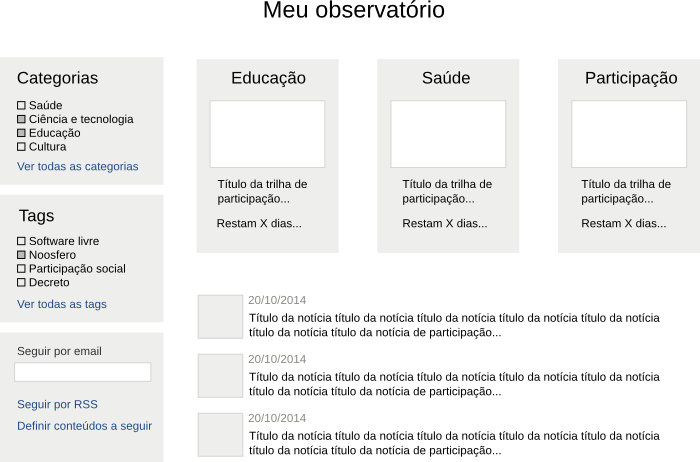
\includegraphics[scale=0.60]{observatorio.png}
\caption{Observatório do Participa.br}
\label{observatorio}
\end{figure}

Com isto cada usuário cadastrado no Participa.br poderá acompanhar
notícias, trilhas, eventos, posts de blog, galeria de imagens, vídeos e
diversos outros tipos de conteúdo existentes na plataforma, recebendo
notificações sempre que forem criados ou atualizados.

\paragraph{Especificação da funcionalidade} \

\

O Participa.br organiza seus debates em torno de comunidades temáticas criadas
a partir do interesse da sociedade ou governo. A gestão das comunidades é
conjunta. A construção de um processo participativo dentro de uma comunidade
ocorre através de criação de diversos tipos de conteúdos e ferramentas
digitais de participação. Estes conteúdos e ferramentas podem ser criados por
qualquer usuário do ambiente participativo e possuem em comum 2 informações de
vital importancia para dar sustentação ao {\it Observatório} aqui proposto, são
elas: tags e categorias (ver Figura~\ref{categorias-tags}), elas dão um viés
estrutural a todo conteúdo e ferramenta de participação criada no
Participa.br.

\begin{figure}[h!]
\center
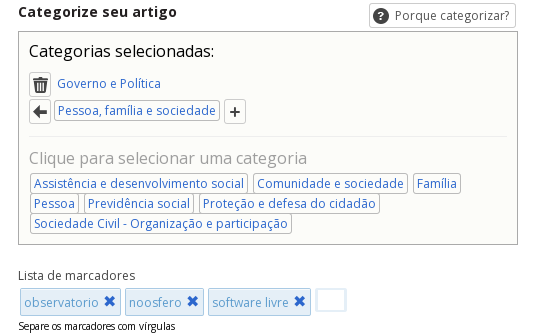
\includegraphics[scale=0.6]{categorias-tags.png}
\caption{Definição de categoria e tag na edição de conteúdo}
\label{categorias-tags}
\end{figure}

A seleção de tags e categorias é um recurso já disponível hoje no Participa.br
e pode ser utilizado em qualquer tipo de conteúdo: artigos texto,
eventos, fóruns, trilhas de participação, posts de blog, galeria de imagens,
vídeos, etc. Uma vez definindo-se tags e categorias para um certo conteúdo, são
gerados links na visualização do mesmo para que os usuários possam navegar no
conteúdo do ambiente através de filtros por tags ou categorias.

A personalização do {\it Observatório} é feita através da seleção de tags e
categorias, esta funcionalidade não está disponível no Participa.br ainda e
deverá ser implementada como proposto nas Figuras \ref{observatorio-tags} e
\ref{observatorio-categorias}. Esta seleção, como demonstrado na
figura~\ref{observatorio-tags}, é realizada através da ação {\bf seguir}, ou
seja, clicar em {\it +seguir tag 'arena net mundial'} significa marcar e
selecionar esta tag como um tema de interesse que será posteriormente
utilizado para compor o conteúdo exibido no {\it Observatório}.

\begin{figure}[h!]
\center
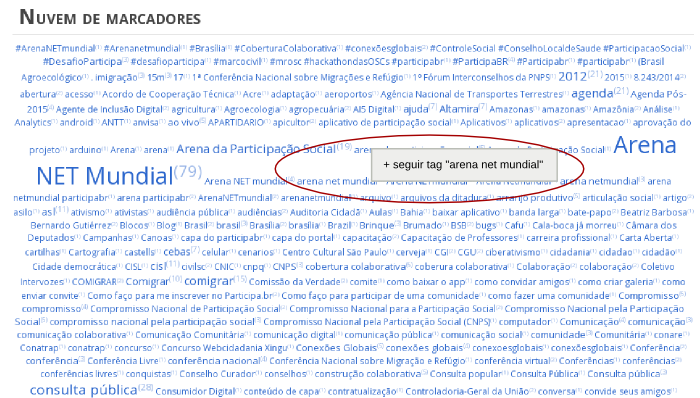
\includegraphics[scale=0.5]{observatorio-seguir-tags.png}
\caption{Seleção de tags para acompanhar no observatório}
\label{observatorio-tags}
\end{figure}

\begin{figure}[h!]
\center
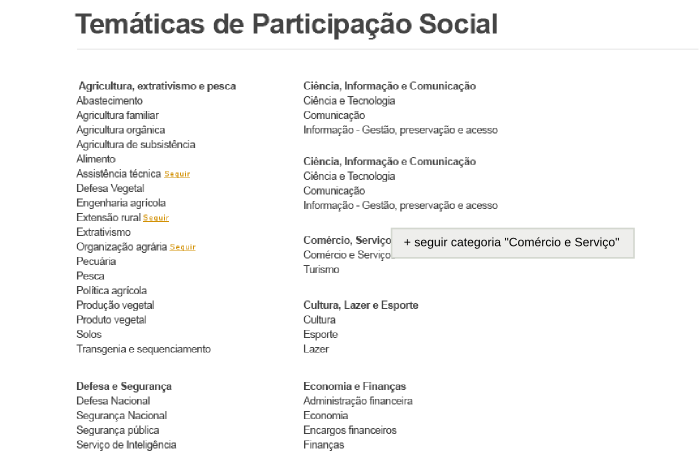
\includegraphics[scale=0.5]{observatorio-categoria.png}
\caption{Seleção de categorias para acompanhar no observatório}
\label{observatorio-categorias}
\end{figure}

O {\it Observatório} será um agregador de conteúdos, cada usuário irá selecionar
temas de seu interesse, esta seleção será armazenada no perfil do usuário na
forma de uma lista de tags e categorias a seguir, esta lista será armazenada
de forma persistente no perfil do usuário de forma que se mantenha sempre que
acesse o Participa.br.

Os usuários poderão acompanhar o {\it Observatório} através de um leitor de
feed\cite{rss} externo (ver Figura~\ref{observatorio-feed}). Isto irá
potencializar a distribuição de conteúdos do Participa.br pois dará a
possibilidade de acessar conteúdos sem necessidade de acesso direto ao
Participa.br.

\begin{figure}[h!]
\center
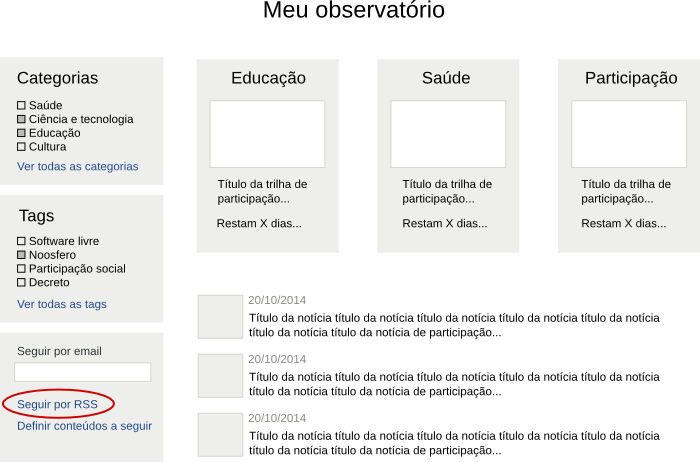
\includegraphics[scale=0.60]{observatorio-feed.png}
\caption{Seguir o observatório via feed RSS}
\label{observatorio-feed}
\end{figure}

Será possível também acompanhar o observatório através do email, o usuário
poderá inscrever um email ou usar o próprio email cadastrado no Participa.br
para receber atualizações do observatório, assim o usuário será notificado
sobre todo conteúdo criado com base nas suas preferências, isso irá disparar
um email por dia com um resumo de todas as novidades.

\begin{figure}[h!]
\center
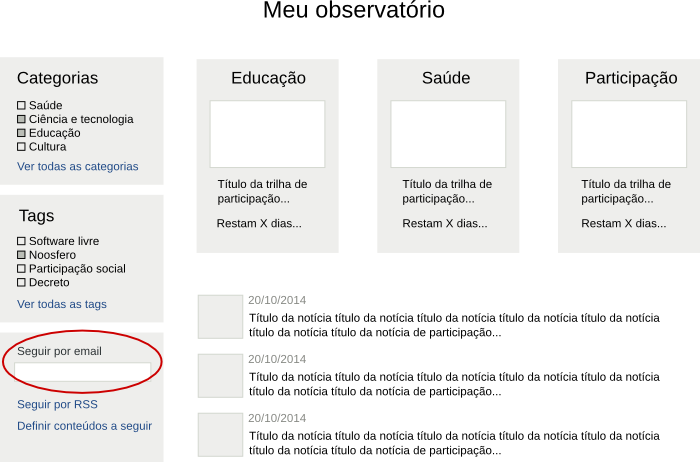
\includegraphics[scale=0.60]{observatorio-email.png}
\caption{Seguir o observatório via email}
\label{observatorio-email}
\end{figure}

O observatório terá suporte também em dispositivos móveis, através de um app
(ver Figura~\ref{observatorio-mobile}) para smartphones, os usuários poderão
interagir com o {\it Observatório} visualizando trilhas, artigos e todos os outros
tipos de conteúdos disponível no observatório, este app fará acesso à API do
Noosfero (ver proposta de API no apendice \ref{api}), esta API irá expor todos
os dados do observatório. Este app irá também notificar os usuários a cada
atualização no observatório de forma que o usuário consiga acompanhar em tempo
real tudo o que acontece.

\begin{figure}[h!]
\center
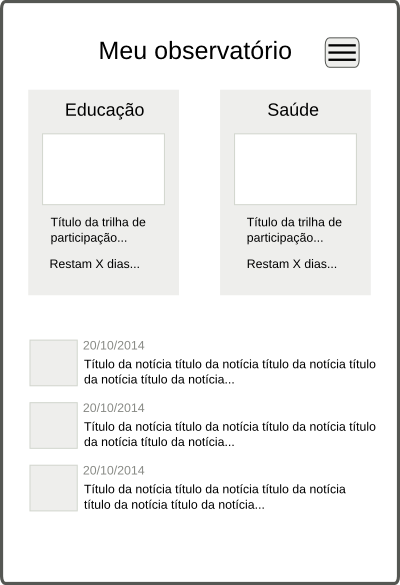
\includegraphics[scale=0.50]{observatorio-mobile.png}
\caption{Proposta de tela para observatório mobile}
\label{observatorio-mobile}
\end{figure}

\begin{figure}[h!]
\center
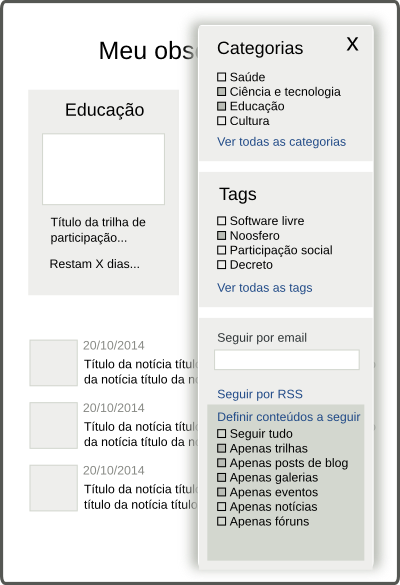
\includegraphics[scale=0.50]{observatorio-mobile-opcoes.png}
\caption{Configuração do observatório mobile}
\label{observatorio-mobile-opcoes}
\end{figure}

Por fim é importante destacar que o observatório irá dar um destaque às
trilhas de participação social, possibilitando acompanhar todas as novidades
que ocorrem nas trilhas de participação, os usuários serão notificados a cada
nova etapa que se inicia ou finaliza, este tratamento especial às datas de
início e fim de cada etapa possibilitará um acompanhamento detalhado de cada
atividade.

Os usuário poderão também acompanhar apenas atualizações ocorridas nas trilhas
se assim desejar, pois será possível escolher quais tipos de conteúdo seguir
(ver Figura~\ref{observatorio-conteudo}), será possível por exemplo dizer que
se quer acompanhar somente trilhas, ou somente posts de blog, ou apenas
galeria de imagens, etc.

\begin{figure}[h!]
\center
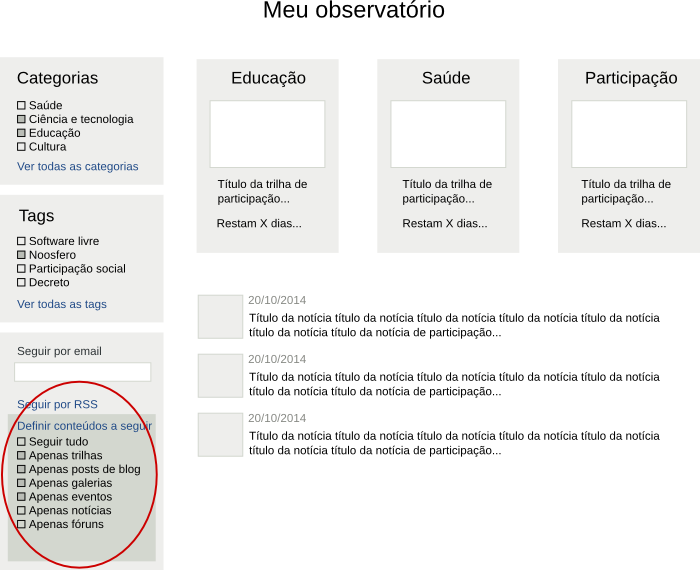
\includegraphics[scale=0.5]{observatorio-tipos-conteudo.png}
\caption{Seleção de tipos de conteúdos para seguir no observatório}
\label{observatorio-conteudo}
\end{figure}

Esta ferramenta irá proporcionar aos usuários uma visão geral e sempre
atualizada de tudo que ocorre no Participa.br, possibilitando acompanhar as
atualizações através de interface diferenciadas, como: email, web, rss,
dispositivos móveis, etc. O apendice~\ref{codigo-observatorio} traz um exemplo
de código para implementação da interface Web do observatório.

\paragraph{Detalhes de implementação} \

\

Segue uma breve descrição de tudo que precisa ser implementado para construir
o {\it Observatório} do Participa.br:

\begin{description}
  \item[Tela principal do Observatório do Participa.br]{Desenvolver uma nova
    interface de usuário para exibir e listar conteúdos com base nas
    preferências do usuário (Figura \ref{observatorio}).}
  \item[Tela para listar todas as categorias do Participa.br]{O Participa.br
    tem inúmeras categorias cadastradas, mas não há uma interface para os
    usuários navegarem nestas categorias, então é preciso desenvolver uma tela
    que exiba de forma organizada todas as categorias cadastradas (Figura
    \ref{observatorio-categorias}).}
  \item[Funcão de "seguir" tags e categorias]{Implementar um botão ou link ao
    lado de cada categoria ou tag que ao ser clicado adicione o item
    na lista de preferências do usuário, indicando que tal tag ou categoria
    representa um tema de seu interesse (Figura \ref{observatorio-tags}).}
  \item[Criar novos campos no perfil de usuário]{Criar novos campos para
      armazenar a lista de categorias e tags, quais tipos de conteúdos está
      seguindo, se quer receber notificação por email.}
  \item[Gerar feed RSS com conteúdos do Observatório]{Implementar uma
    funcionalidade para compor uma fonte RSS a partir dos dados do
    Observatório do usuário, este RSS é específico para cada usuário, pois deve
    levar em consideração as preferências individuais de cada um.}
  \item[Aplicativo módel para Observatório]{Aplicativo utilizando tecnologias
    Web (HTML, Javascript, CSS) para exibir e notificar sobre as atualizações
    do Participa.br, este aplicativo deve ser desenvolvido utilizando
    tecnologias que permitam rodar em diversar plataformas (Android, iPhone, etc)
    (Figuras \ref{observatorio-mobile} e \ref{observatorio-mobile-opcoes}).}
  \item[API para aplicativo móvel]{O aplicativo móvel precisará de acesso a
    uma API do Participa.br de forma a fornecer os dados necessários para
    compor as funcionalidades do app móvel, o Participa.br possui uma API, esta
    API precisará ser evoluída para fornecer mais alguns dados como exemplificado
    no apendice \ref{api}.}
  \item[Acompanhar Observatório por email]{Será preciso desenvolver um serviço
    que fique constantemente acompanhando as atualizações de conteúdo do
    Participa.br e notifique cada usuário do Observatório de acordo suas
    preferências, este serviço poderá ser implementado como um novo {\it daemon},
    semelhante ao {\it feed-updater} já existente.}
\end{description}

\subsubsection{Painel gestor das ferramentas de consulta}

O {\it Painel gestor} é uma proposta de nova funcionalidade contendo um painel
administrativo de sistematização de consultas com base nas ferramentas de
comentários por trecho e por parágrafo usando etiquetas e status, definidos
dinamicamente via interface administrativa.

Esta proposta de ferramenta de sistematização prevê o uso do plugin Noosfero
CommentClassification\cite{commentClassificationPlugin}, este plugin
possibilita classificar comentários através de etiquetas e status, ele foi
desenvolvido pela consultora PNUD Daniela Feitosa como
parte da pesquisa para elaboração do Produto 04, a partir
deste plugin os usuários podem indicar semanticamente qual o significado do
seu comentário no momento em que o faz, veja exemplo de uso na
Figura~\ref{etiqueta}.

\begin{figure}[h!]
\center
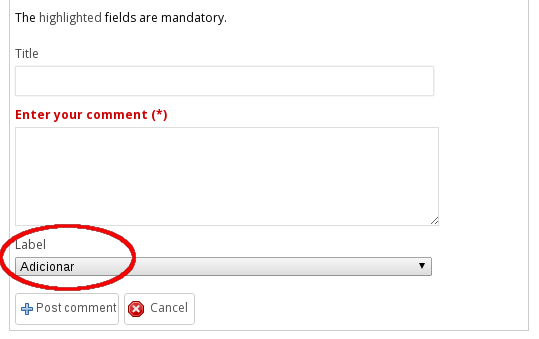
\includegraphics[scale=0.5]{etiqueta.png}
\caption{Etiquetas de classificação para comentários}
\label{etiqueta}
\end{figure}

Apesar do plugin possibilitar seleção de etiquetas e status nos comentários,
estas informações não são utilizadas para nada, este plugin ou nenhum outro
oferece nenhuma utilidade para as etiquetas e status marcados em cada
comentário.

A funcionalidade descrita aqui propõe, então, uma forma de utilizar as
informações de etiquetas e status associadas aos comentários com objetivo de
sistematizar e analisar os resultados de consultas públicas através de
ferramentas de comentários por trecho ou por parágrafo, ou seja, consultas que
usem esta ferramenta terão uma forma simplificada de analisar e agregar as
contribuições dos usuários realizadas através dos comentários.

\paragraph{Especificação da funcionalidade} \

\

O administrador da consulta deve cadastrar etiquetas e status a partir do
painel de controle administrativo do ambiente como pode ser visto nas Figuras
\ref{manage-labels} e \ref{manage-status}, criando uma lista de opções para
cada campo. O administrador pode por exemplo criar etiquetas que indiquem:

\begin{itemize}
  \item Adição ou remoção de texto
  \item Concordancia ou discordancia
  \item Opinião sobre qualidade do texto (bom, ruim, etc)
\end{itemize}

\begin{figure}[h!]
\center
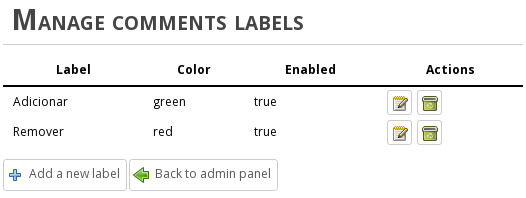
\includegraphics[scale=0.5]{manage-labels.png}
\caption{Gerenciamento de labels do plugin CommentClassification}
\label{manage-labels}
\end{figure}

Esta funcionalidade de cadastrar etiquetas e status já está presente no plugin
e portanto já disponível no Participa.br.

\begin{figure}[h!]
\center
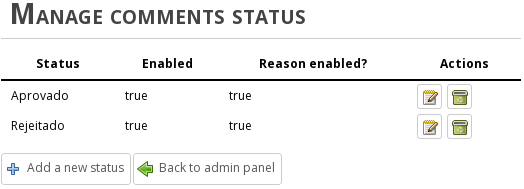
\includegraphics[scale=0.5]{manage-status.png}
\caption{Gerenciamento de status do plugin CommentClassification}
\label{manage-status}
\end{figure}

Cada etiqueta pode ter uma cor associada, desta forma pode-se diferenciar
visualmente os comentários a partir da etiqueta selecionada.

As etiquetas podem ser utilizadas por qualquer usuário mas o status é
utilizado apenas pelos avaliadores enquanto analisam os comentários. Estes
avaliadores são usuários com papel específico e permissão de marcar status
num comentário, vários avaliadores podem marcar diferentes status num
mesmo comentário, estas informações serão utilizadas pelo administrador da consulta
ao avaliar o que irá considerar ou descartar em cada comentário.

Tanto os avaliadores quando o administrador de uma consulta podem gerenciar
comentários definindo status para eles a partir do painel de controle (ver
Figura~\ref{control-panel}).

\begin{figure}[h!]
\center
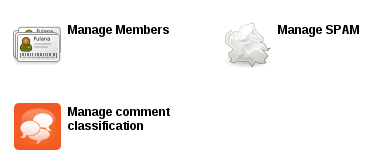
\includegraphics[scale=0.5]{control-panel.png}
\caption{Imagem no painel de controle da comunidade}
\label{control-panel}
\end{figure}

Assim como é feito para as etiquetas, o administrador deve cadastrar
previamente os status através da configuração do plugin no painel do
administrador (ver Figura~\ref{manage-status}). Exemplos:

\begin{itemize}
  \item Recomento
  \item Não recomendo
  \item Boa proposta
  \item Proposta ruim
\end{itemize}

Cada trecho ou parágrafo de um texto em uma consulta pode ter vários
comentários, cada comentário tem uma etiqueta indicando a semântica dele, cada
comentário poderá receber vários status pelos avaliadores. O
administrador da consulta irá utilizar estas informações para elaborar uma
nova proposta do texto com base nas contribuições dos usuários, ver Figuras
\ref{manage-comments} e \ref{manage-comments-commit} com a proposta de interface
para esta funcionalidade.

\begin{figure}[h!]
\center
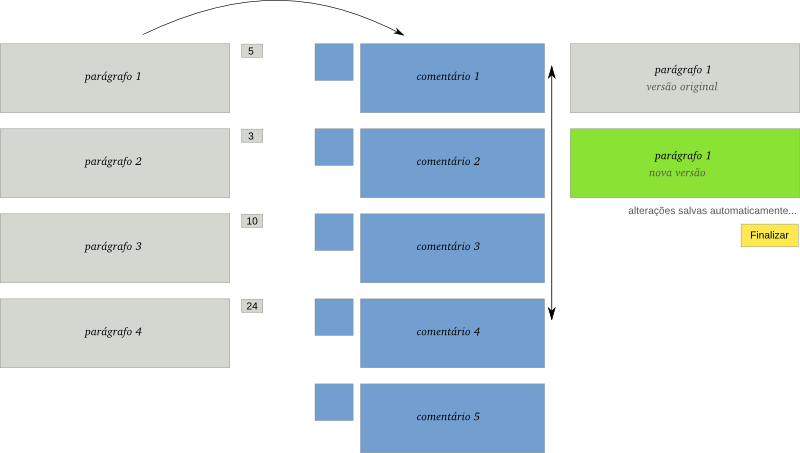
\includegraphics[scale=0.3]{manage-comments.png}
\caption{Revisão de comentários, etiquetas e status}
\label{manage-comments}
\end{figure}

\begin{figure}[h!]
\center
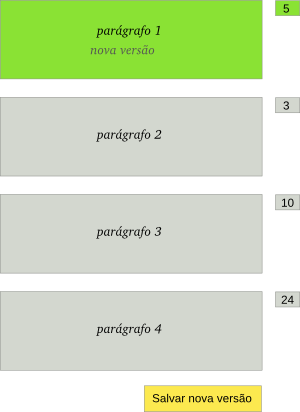
\includegraphics[scale=0.3]{manage-comments-commit.png}
\caption{Finalizar revisão de comentários, etiquetas e status}
\label{manage-comments-commit}
\end{figure}

O painel de controle de gestão deve disponibilizar uma opção de exportação em
CSV dos trechos, comentários, status e etiquetas de forma que seja possível
analisar tais dados externamente a partir de ferramentas de análise (ver
exemplo de código no apendice \ref{csv}).

Ao finalizar a revisão dos comentários (Figura \ref{manage-comments-commit}) uma
nova versão do texto da consulta é gerada, isto será possibilitado pela
infra-estrutura de controle versões de artigos do Noosfero, assim cada vez que
o administrador analisar os comentários e agregar eles numa nova proposta de
texto, uma nova versão do artigo será gerado, desta forma preservando o
texto original ao ponto que gera um novo a partir das contribuições dos
usuários. Assim será possível acompanhar todo o histórico de mudanças de um
artigo.

Além de possibilitar manipular o texto de uma consulta a partir das
contribuições dos usuário em forma de comentários, esta ferramenta deverá
também gerar estatísticas sobre as contribuições dos usuários, por
exemplo: quantos usuário querem adicionar conteúdo, quantos querem suprimir,
quais os questionamentos sobre o texto, quais os status marcados pelos
avaliadores, quantas avaliações cada comentário recebeu, etc.

Esta ferramenta de sistematização irá proporcionar meios e informações
suficientes para dar suporte ao administrador de uma consulta em analisar e
avaliar as contribuições dos usuários feitos a partir de comentários em um
texto de consulta, com o objetivo final de agregar tais contribuições num novo
texto mantendo todo o histórico de alterações realizado.

\paragraph{Detalhes de implementação} \

\

Segue uma breve descrição de tudo que precisa ser implementado para construir
{\it Painel gestor das ferramentas de consulta} do Participa.br:

\begin{description}
  \item[Mostrar etiquetas na visualização dos comentários]{As etiquetas
    selecionadas pelos usuários no momento do comentário não são exibidas em
    lugar algum após terem sido feitas, será preciso alterar a implementação da
    visualização de comentários para levar em consideração este campo exibindo
    ele de forma adequada.}
  \item[Mostrar status na visualização e gestão de comentários]{Mais de um
    avaliador pode definir status para um mesmo comentário, desta forma um
    único comentário poderá ter vários status, será preciso evoluir a interface
    de visualização de comentários para exibir esta informação
    aos administradores apenas, pois somente usuários com perfil de administrador
    podem visualizar os status marcados pelos avaliadores.}
  \item[Interface principal de sistematização de consultas]{Será preciso
    desenvolver uma interface administrativa para possibilitar o
    administrador manipular os parágrafos de um texto em consulta, de forma que
    seja possível visualizar facilmente as etiquetas e status definidos pelos
    usuários e avaliadores. Esta interface irá exibir o texto em consulta de
    um lado e os comentários do outro, como mostra a Figura
    \ref{manage-comments}, de forma que a cada parágrafo revisado seja marcado
    com um status indicando que tal parágrafo foi revisado. Esta nova
    interface deve possibilitar que o administrador revise e sistematize um novo
    texto para cada parágrafo individualmente.}
  \item[Administrador gera nova versão do texto com base nos comentários]{Nova
    funcionalidade que permita gerar uma nova versão do texto após revisão das
    etiquetas e status, esta nova versão do texto terá como base as
    contribuições dos usuários através de seus comentários, uma nova consulta
    poderá ser aberta após a sistematização feita pelo administrador,
    possibilitando um processo incremental de consulta com base num texto base
    inicial.}
  \item[Definir status em parágrafo indicando que foi
    sistematizado/revisado pelo administrador]{Será preciso criar um novo
    campo associado a cada parágrafo de um artigo texto, este status irá
    receber uma indicação de que o administrador já o revisou, este status será
    utilizado na visualização dos parágrafos, os já revisados serão exibidos numa
    cor diferente. Esta diferenciação estará disponível apenas para
    administradores e avaliadores (Figura \ref{manage-comments-commit}).}
  \item[Exportar dados associados aos comentários em formato CSV]{Os
    comentários e suas respectivas etiquetas e status devem ser exportados
    para um arquivo CSV, então será preciso implementar uma funcionalidade nova
    que percorra todos os comentários e gere um CSV contendo: conteúdo do
    comentário, autor do comentário, data, etiqueta e todos os status associados e
    seus respectivos avaliadores.}
  \item[Interface de exibição de estatísticas de contribuições]{Implementar
    uma interface para exibir estatísticas da consulta, exibindo quantos
    usuários querem adicionar conteúdo, quantos querem remover, quantos
    concordam com o texto da consulta, quantos discordam, quantas avaliações
    cada comentário recebeu por parte dos avaliadores.}
\end{description}

\section{Conclusão}

Neste documento foi apresentado um \ProductDescription

Lembramos que para tornar o Portal de Consulta Pública realmente um canal de
consulta e participação popular na discussão e na definição da agenda
prioritária do país, é necessário que além de documentação faça-se um esforço
de movimentar as pessoar fora do ambiente virtual, para que haja um
engajamento no uso e contribuição deste projeto de forma consistente e perene.

\newpage
\bibliography{bibliografia}
\newpage
\listoffigures
\newpage
\printindex
\newpage
\definecolor{lightgrey}{rgb}{0.95,0.95,0.95}
\lstset{language=Ruby,basicstyle=\small\ttfamily,backgroundcolor=\color{lightgrey}}

\section{Anexos}

\subsection{Exemplo de código do plugin Noosfero para pairwise}

\lstinputlisting{pairwise_content.rb}

\subsection{Exemplo de código XML retornado pelo pairwise-api}

\begin{lstlisting}
<?xml version="1.0" encoding="UTF-8"?>
<prompt>
  <created-at type="datetime">2010-07-01T23:48:01+00:00</created-at>
  <id type="integer">1</id>
  <left-choice-id type="integer">10</left-choice-id>
  <question-id type="integer">7</question-id>
  <right-choice-id type="integer">9</right-choice-id>
  <tracking nil="true"></tracking>
  <updated-at type="datetime">2010-07-01T23:48:01+00:00</updated-at>
  <votes-count type="integer">0</votes-count>
  <left-choice-text>bar</left-choice-text>
  <right-choice-text>foo</right-choice-text>
</prompt>
\end{lstlisting}

\appendix
\appendixpage
\section{Foo bar}
\label{foobar}

%\lstinputlisting{observatorio.rb}


\end{document}
